% ---------------------------------------------------------------------------
% Quelle der Abbildung:
%   Skript:  thesis/figures/scripts/ctf_kurven.py (analytisch, kein Trainingslauf)
%   Aufruf:  /tmp/holo311/bin/python thesis/figures/scripts/ctf_kurven.py
%   Basis:   Commit 1abccf9 (Branch cursor/thesis-grundlagen-6175), 2026-10-01
%   Dateien: ctf_kurven.pdf
% Einbinden im Kapitel: % ---------------------------------------------------------------------------
% Quelle der Abbildung:
%   Skript:  thesis/figures/scripts/ctf_kurven.py (analytisch, kein Trainingslauf)
%   Aufruf:  /tmp/holo311/bin/python thesis/figures/scripts/ctf_kurven.py
%   Basis:   Commit 1abccf9 (Branch cursor/thesis-grundlagen-6175), 2026-10-01
%   Dateien: ctf_kurven.pdf
% Einbinden im Kapitel: % ---------------------------------------------------------------------------
% Quelle der Abbildung:
%   Skript:  thesis/figures/scripts/ctf_kurven.py (analytisch, kein Trainingslauf)
%   Aufruf:  /tmp/holo311/bin/python thesis/figures/scripts/ctf_kurven.py
%   Basis:   Commit 1abccf9 (Branch cursor/thesis-grundlagen-6175), 2026-10-01
%   Dateien: ctf_kurven.pdf
% Einbinden im Kapitel: % ---------------------------------------------------------------------------
% Quelle der Abbildung:
%   Skript:  thesis/figures/scripts/ctf_kurven.py (analytisch, kein Trainingslauf)
%   Aufruf:  /tmp/holo311/bin/python thesis/figures/scripts/ctf_kurven.py
%   Basis:   Commit 1abccf9 (Branch cursor/thesis-grundlagen-6175), 2026-10-01
%   Dateien: ctf_kurven.pdf
% Einbinden im Kapitel: \input{figures/grundlagen/ctf_kurven}
% ---------------------------------------------------------------------------
\begin{figure}[tb]
  \centering
  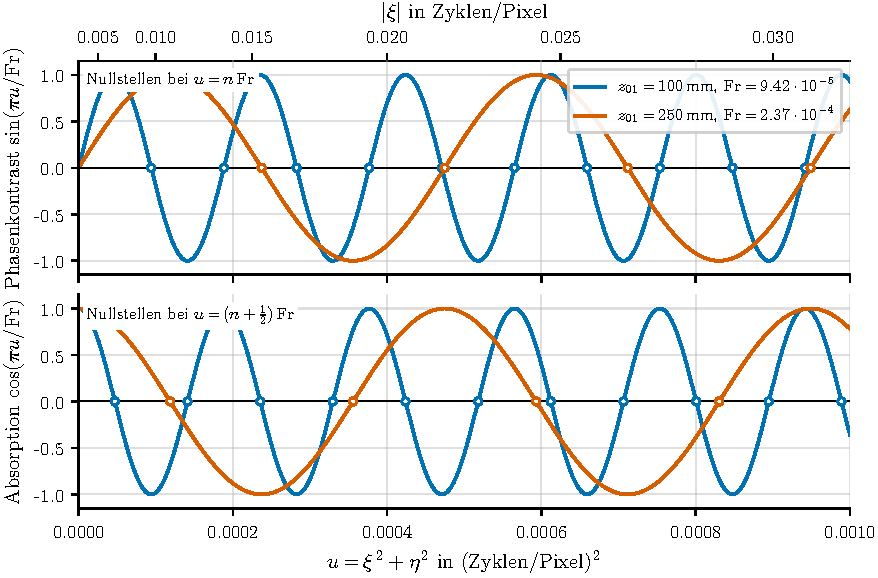
\includegraphics[width=\textwidth]{figures/grundlagen/ctf_kurven}
  \caption[Kontrastübertragungsfunktion schwacher Objekte für zwei Fresnel-Zahlen]{%
    Kontrastübertragungsfunktion schwacher Objekte nach
    \cref{eq:grundlagen:ctf} über $u = \xi^2+\eta^2$ für zwei Fresnel-Zahlen der
    P05-Standardgeometrie (\qty{11}{\kilo\electronvolt}, $\zTwo = \qty{20}{\metre}$,
    $\dx = \qty{6.5}{\micro\metre}$): $\zOne = \qty{100}{\milli\metre}$
    ($\Fr = \num{9.42e-5}$) und $\zOne = \qty{250}{\milli\metre}$
    ($\Fr = \num{2.37e-4}$). Oben der Phasenkontrast $\sin(\pi u/\Fr)$ mit
    Nullstellen bei $u = n\,\Fr$, unten der Absorptionskontrast $\cos(\pi u/\Fr)$
    mit Nullstellen bei $u = (n+\tfrac12)\,\Fr$ (Kreise). Die Nullstellen liegen in
    $u$ äquidistant mit Abstand $\Fr$; ihre Lage ist die spektrale Signatur der
    Fresnel-Zahl.}
  \label{fig:grundlagen:ctf}
\end{figure}

% ---------------------------------------------------------------------------
\begin{figure}[tb]
  \centering
  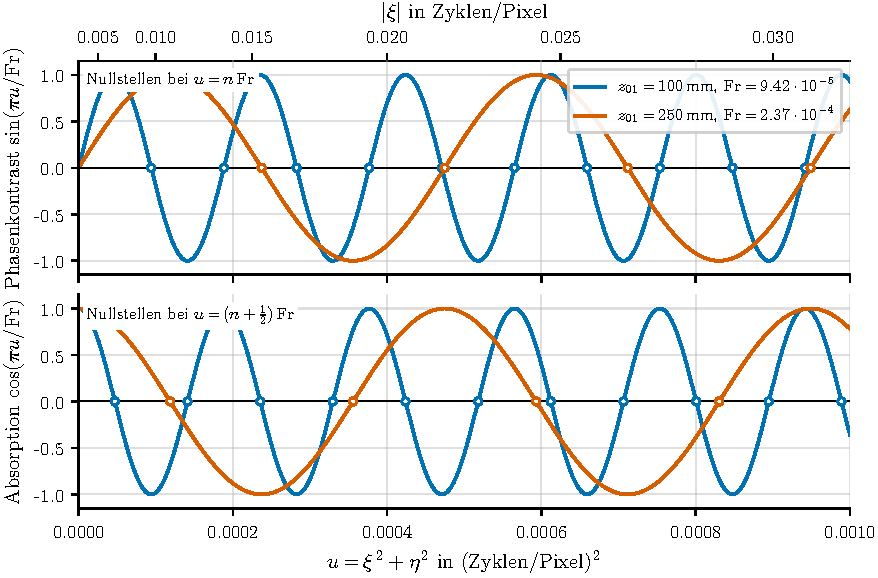
\includegraphics[width=\textwidth]{figures/grundlagen/ctf_kurven}
  \caption[Kontrastübertragungsfunktion schwacher Objekte für zwei Fresnel-Zahlen]{%
    Kontrastübertragungsfunktion schwacher Objekte nach
    \cref{eq:grundlagen:ctf} über $u = \xi^2+\eta^2$ für zwei Fresnel-Zahlen der
    P05-Standardgeometrie (\qty{11}{\kilo\electronvolt}, $\zTwo = \qty{20}{\metre}$,
    $\dx = \qty{6.5}{\micro\metre}$): $\zOne = \qty{100}{\milli\metre}$
    ($\Fr = \num{9.42e-5}$) und $\zOne = \qty{250}{\milli\metre}$
    ($\Fr = \num{2.37e-4}$). Oben der Phasenkontrast $\sin(\pi u/\Fr)$ mit
    Nullstellen bei $u = n\,\Fr$, unten der Absorptionskontrast $\cos(\pi u/\Fr)$
    mit Nullstellen bei $u = (n+\tfrac12)\,\Fr$ (Kreise). Die Nullstellen liegen in
    $u$ äquidistant mit Abstand $\Fr$; ihre Lage ist die spektrale Signatur der
    Fresnel-Zahl.}
  \label{fig:grundlagen:ctf}
\end{figure}

% ---------------------------------------------------------------------------
\begin{figure}[tb]
  \centering
  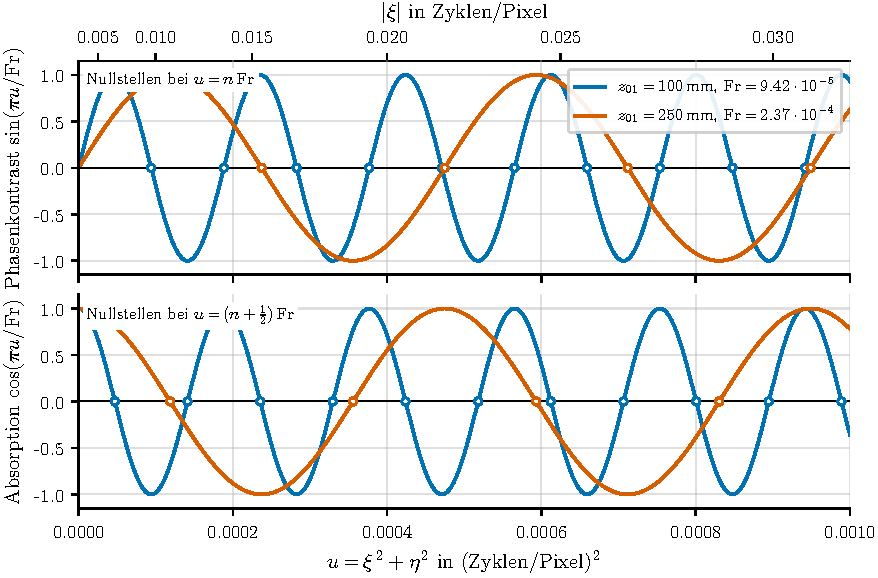
\includegraphics[width=\textwidth]{figures/grundlagen/ctf_kurven}
  \caption[Kontrastübertragungsfunktion schwacher Objekte für zwei Fresnel-Zahlen]{%
    Kontrastübertragungsfunktion schwacher Objekte nach
    \cref{eq:grundlagen:ctf} über $u = \xi^2+\eta^2$ für zwei Fresnel-Zahlen der
    P05-Standardgeometrie (\qty{11}{\kilo\electronvolt}, $\zTwo = \qty{20}{\metre}$,
    $\dx = \qty{6.5}{\micro\metre}$): $\zOne = \qty{100}{\milli\metre}$
    ($\Fr = \num{9.42e-5}$) und $\zOne = \qty{250}{\milli\metre}$
    ($\Fr = \num{2.37e-4}$). Oben der Phasenkontrast $\sin(\pi u/\Fr)$ mit
    Nullstellen bei $u = n\,\Fr$, unten der Absorptionskontrast $\cos(\pi u/\Fr)$
    mit Nullstellen bei $u = (n+\tfrac12)\,\Fr$ (Kreise). Die Nullstellen liegen in
    $u$ äquidistant mit Abstand $\Fr$; ihre Lage ist die spektrale Signatur der
    Fresnel-Zahl.}
  \label{fig:grundlagen:ctf}
\end{figure}

% ---------------------------------------------------------------------------
\begin{figure}[tb]
  \centering
  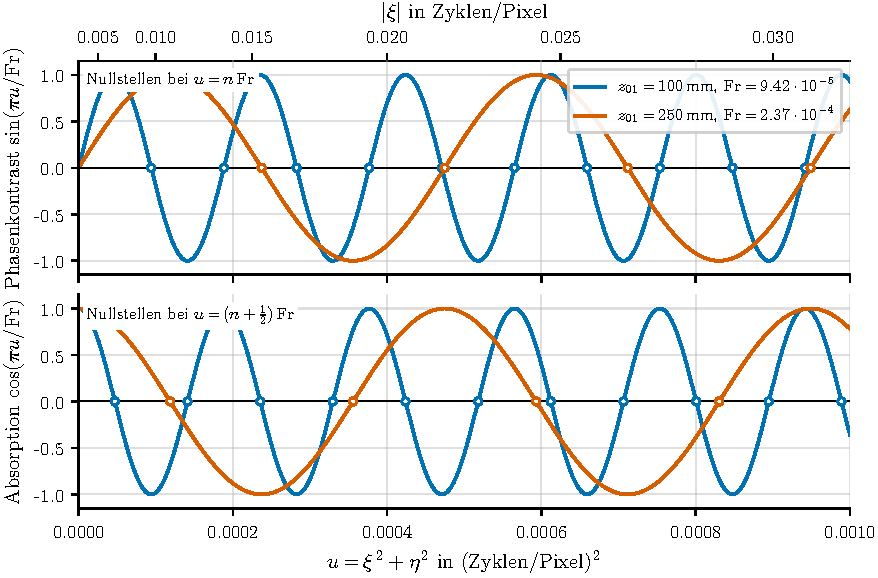
\includegraphics[width=\textwidth]{figures/grundlagen/ctf_kurven}
  \caption[Kontrastübertragungsfunktion schwacher Objekte für zwei Fresnel-Zahlen]{%
    Kontrastübertragungsfunktion schwacher Objekte nach
    \cref{eq:grundlagen:ctf} über $u = \xi^2+\eta^2$ für zwei Fresnel-Zahlen der
    P05-Standardgeometrie (\qty{11}{\kilo\electronvolt}, $\zTwo = \qty{20}{\metre}$,
    $\dx = \qty{6.5}{\micro\metre}$): $\zOne = \qty{100}{\milli\metre}$
    ($\Fr = \num{9.42e-5}$) und $\zOne = \qty{250}{\milli\metre}$
    ($\Fr = \num{2.37e-4}$). Oben der Phasenkontrast $\sin(\pi u/\Fr)$ mit
    Nullstellen bei $u = n\,\Fr$, unten der Absorptionskontrast $\cos(\pi u/\Fr)$
    mit Nullstellen bei $u = (n+\tfrac12)\,\Fr$ (Kreise). Die Nullstellen liegen in
    $u$ äquidistant mit Abstand $\Fr$; ihre Lage ist die spektrale Signatur der
    Fresnel-Zahl.}
  \label{fig:grundlagen:ctf}
\end{figure}
